
\documentclass[12pt]{article}
\usepackage{babel}
\usepackage[utf8]{inputenc}
\usepackage[T1]{fontenc}
\usepackage{geometry}
\usepackage{booktabs}
\usepackage{tabularx}
\usepackage{float}
\usepackage{array}
\usepackage{graphicx}
\graphicspath{{img/}}
\geometry{a4paper, margin=2cm}
\title{Sprawozdanie z projektu \\ \large,,Wpływ warunków pogodowych na rynek energii elektrycznej w Polsce''}
\author{Dubois Jozef, Gajda Stefan (Neandertalczycy SQLa)}
\date{}
\sloppy
\begin{document}

	\maketitle


	\section{Tematyka i cel biznesowy}

	Celem projektu jest zaprojektowanie hurtowni danych oraz warstwy raportowej pozwalającej analizować wpływ warunków pogodowych na pracę systemu elektroenergetycznego w Polsce. System integruje dane pogodowe, dane o produkcji energii przez jednostki wytwórcze oraz dane ogólnokrajowe dotyczące cen, bilansu i zapotrzebowania na energię elektryczną. Rozwiązanie umożliwia analizę zależności między temperaturą, wiatrem, opadami, ciśnieniem i innymi parametrami pogodowymi a obciążeniem KSE, produkcją elektrowni oraz cenami energii.

	\textbf{Cel biznesowy:}
	\begin{itemize}
		\item identyfikacja czynników pogodowych wpływających na zmienność zapotrzebowania na energię elektryczną,
		\item analiza zależności między warunkami pogodowymi a produkcją poszczególnych elektrowni,
		\item porównanie prognozowanego i rzeczywistego obciążenia krajowego systemu elektroenergetycznego,
		\item monitorowanie cen energii i ich powiązania z bilansem mocy oraz pogodą,
		\item wsparcie analityków w ocenie sezonowości, ryzyka pogodowego i odchyleń od typowego profilu pracy systemu.
	\end{itemize}

	\textbf{Planowane korzyści z perspektywy odbiorcy rozwiązania:}
	\begin{itemize}
		\item szybszy dostęp do zintegrowanych danych z wielu źródeł w jednym modelu hurtowni,
		\item możliwość porównywania danych pogodowych, produkcyjnych i cenowych w tej samej granularności czasowej,
		\item lepsze zrozumienie wpływu ekstremalnych temperatur, wiatru lub opadów na zużycie i ceny energii,
		\item łatwiejsze przygotowanie raportów dla kierownictwa, analityków rynku energii oraz zespołów planowania produkcji,
		\item ograniczenie ręcznej pracy związanej z pobieraniem, czyszczeniem i łączeniem danych z API.
	\end{itemize}

	\textbf{Odbiorcy rozwiązania:}
	\begin{itemize}
		\item analitycy rynku energii,
		\item operatorzy i jednostki planujące pracę systemu elektroenergetycznego,
		\item zespoły odpowiedzialne za prognozowanie zapotrzebowania i analizę cen,
		\item osoby przygotowujące raporty zarządcze i operacyjne dotyczące rynku energii.
	\end{itemize}

	\section{Źródła danych}

	W rozwiązaniu wykorzystywane są dwa źródła pobierane cyklicznie przez API (PSE oraz Meteostat) oraz jedno źródło referencyjne w postaci kuratorowanego pliku CSV z metadanymi elektrowni. Lista jednostek wytwórczych pochodzi z PSE, ich atrybuty opisowe (kategoria, moc, lokalizacja, województwo) są utrzymywane w pliku \texttt{powerplant\_meta.csv}, a same atrybuty pochodzą z bazy elektrowni serwisu Instrat.

	\subsection{Dane energetyczne - PSE API}
	\begin{itemize}
		\item Źródło: \texttt{https://api.raporty.pse.pl/api/}
		\item Wykorzystywane obszary danych:
		\begin{itemize}
			\item \texttt{gen-jw} - dane o generacji jednostek wytwórczych (oraz lista elektrowni),
			\item \texttt{energy-prices} - dane cenowe i bilansowe,
			\item \texttt{rce-pln} - rynkowa cena energii,
			\item \texttt{kse-load} - prognozowane i rzeczywiste zapotrzebowanie KSE.
		\end{itemize}
		\item Format danych: odpowiedzi REST w formacie JSON, z obsługą paginacji (pole \texttt{nextLink}).
		\item Częstotliwość odświeżania: dziennie, dla zamkniętego okna dat (domyślnie od dwóch miesięcy wstecz do dnia poprzedniego).
		\item Docelowe tabele: \texttt{FactPowerPlantOutput}, \texttt{FactPolandEnergy} oraz lista elektrowni do \texttt{DimPowerPlant}.
	\end{itemize}

	\subsection{Metadane elektrowni - plik \texttt{powerplant\_meta.csv}}
	\begin{itemize}
		\item Źródło: kuratorowany plik CSV utrzymywany w repozytorium projektu.
		\item Zakres danych: nazwa elektrowni (klucz biznesowy), kategoria/rodzaj paliwa, moc zainstalowana w MW, współrzędne geograficzne, województwo.
		\item Pochodzenie: dla elektrowni występujących w odpowiedziach PSE (endpoint \texttt{gen-jw}) atrybuty opisowe - kategorię/rodzaj paliwa, moc zainstalowaną, współrzędne i województwo - przepisano z bazy elektrowni serwisu Instrat (\texttt{https://energy.instrat.pl/system-elektroenergetyczny/baza-elektrowni/}), uzupełniając w razie potrzeby geokodowanie nazw (usługa Nominatim, wynik zapisany w \texttt{geo\_cache.json}). W bieżącym, cyklicznym procesie ETL nie są wykonywane zapytania do Instrat ani Nominatim - dane czerpane są z pliku CSV.
		\item Częstotliwość aktualizacji: rzadko, ręcznie - po pojawieniu się nowej jednostki w danych PSE lub po zmianie atrybutów elektrowni.
		\item Docelowa tabela: \texttt{DimPowerPlant} (obsługa historii zmian mechanizmem SCD typu 2).
	\end{itemize}

	\subsection{Dane pogodowe - Meteostat API}
	\begin{itemize}
		\item Źródło: \texttt{meteostat.p.rapidapi.com/point/hourly} (dostęp przez RapidAPI, klucz w zmiennej środowiskowej \texttt{RAPIDAPI\_KEY}).
		\item Zakres danych (realnie ładowany): temperatura, punkt rosy, wilgotność względna, opady, kierunek i prędkość wiatru, ciśnienie, kod zjawiska pogodowego.
		\item Format danych: odpowiedź REST w formacie JSON.
		\item Granularność: dane godzinowe dla punktu określonego współrzędnymi elektrowni  pobierane w oknach do 30 dni.
		\item Częstotliwość odświeżania: dziennie. Uwaga: dostawca publikuje dane stacji z kilkudniowym opóźnieniem, co jest uwzględnione w kontroli jakości.
		\item Docelowa tabela: \texttt{FactWeather}.
	\end{itemize}

	\subsection{Zestawienie źródeł danych}

	\begin{table}[h!]
		\centering
		\small
		\begin{tabularx}{\textwidth}{|p{3.0cm}|p{3.1cm}|p{2.1cm}|p{2.4cm}|X|}
			\hline
			\textbf{Źródło} & \textbf{Dane} & \textbf{Format} & \textbf{Odświeżanie} & \textbf{Zastosowanie w modelu} \\
			\hline
			PSE API & produkcja, ceny, bilans, zapotrzebowanie, lista jednostek & JSON/REST & dziennie (okno dat) & zasilenie \texttt{FactPowerPlantOutput} i \texttt{FactPolandEnergy} oraz lista elektrowni \\
			\hline
			\texttt{powerplant\_meta.csv} & kategoria, moc, współrzędne, województwo & CSV & rzadko / ręcznie & atrybuty i SCD2 w \texttt{DimPowerPlant} \\
			\hline
			Meteostat API & pogoda godzinowa dla punktu & JSON/REST & dziennie (z lagiem źródła) & zasilenie \texttt{FactWeather} dla lokalizacji elektrowni \\
			\hline
		\end{tabularx}
		\caption{Źródła danych wykorzystywane w projekcie}
	\end{table}

	\section{Analiza źródeł danych}

	\subsection{Harmonogram odświeżania}
	\begin{itemize}
		\item Jednorazowe pobranie danych historycznych z PSE oraz danych pogodowych dla wybranego zakresu czasu, jednorazowe wygenerowanie wymiaru czasu.
		\item Cykliczne (dzienne) przeładowanie zamkniętego okna dat - domyślnie od dwóch miesięcy wstecz do dnia poprzedniego, bez dnia bieżącego.
		\item Dane pogodowe z Meteostat są pobierane dla współrzędnych aktywnych elektrowni odczytanych z \texttt{DimPowerPlant}.
	\end{itemize}

	\subsection{Identyfikowane problemy}
	\begin{itemize}
		\item różne formaty i nazwy pól w źródłach danych,
		\item konieczność synchronizacji danych czasowych z wielu endpointów PSE,
		\item różne granularności danych: krajowa dla cen i obciążenia, jednostkowa dla produkcji elektrowni oraz punktowa dla pogody,
		\item konieczność mapowania nazw jednostek wytwórczych z PSE do wymiaru elektrowni,
		\item obsługa zmiany czasu letniego i zimowego, czyli godzin brakujących oraz godzin zduplikowanych,
		\item potrzeba utrzymania historii zmian atrybutów elektrowni, np. kategorii lub mocy zainstalowanej,
		\item obsługa paginacji odpowiedzi PSE API,
		\item kilkudniowe opóźnienie publikacji danych pogodowych przez Meteostat.
	\end{itemize}

	\subsection{Niezbędne transformacje}
	\begin{itemize}
		\item ujednolicenie formatów dat i czasu do jednego standardu używanego w hurtowni,
		\item wygenerowanie wymiaru czasu z atrybutami roku, kwartału, miesiąca, tygodnia, dnia, godziny i kwadransa,
		\item oznaczenie dni weekendowych oraz dni zmiany czasu za pomocą pól \texttt{isWeekend}, \texttt{isExtraHourDay}, \texttt{isExtraHour}, \texttt{isMissingHourDay} i \texttt{isMissingHour},
		\item agregacja produkcji po jednostkach wytwórczych do ziarna elektrowni w tabeli \texttt{FactPowerPlantOutput},
		\item agregacja danych krajowych do kwadransa: średnia dla miar cenowych i zapotrzebowania, suma dla bilansu mocy,
		\item lookup kluczy obcych \texttt{TimeId} i \texttt{PowerPlantId},
		\item obsługa historii zmian elektrowni mechanizmem SCD typu 2.
	\end{itemize}

	\section{Architektura rozwiązania}

	System zaprojektowano w architekturze warstwowej. Trzon stanowi hurtownia danych w Microsoft SQL Server. Ekstrakcja i transformacja danych ze źródeł realizowana jest skryptami w języku Python, które zapisują dane do warstwy staging, ładowanie z warstwy staging do modelu wymiarowego (z obsługą SCD2 i lookupów kluczy) wykonują pakiety SSIS. Po przetworzeniu dane są wykorzystywane w raportach Power BI.

	\begin{figure}[h!]
		\centering
		\fbox{%
		\begin{minipage}{0.94\textwidth}
		\centering
		\textbf{Źródła danych}\\[0.15cm]
		PSE API \quad | \quad \texttt{powerplant\_meta.csv} \quad | \quad Meteostat API\\[0.2cm]
		$\Downarrow$\\[0.15cm]
		\textbf{Warstwa ekstrakcji i transformacji - Python}\\
		pobranie JSON/CSV, parsowanie i czyszczenie, agregacja do wspólnego ziarna, obsługa zmiany czasu\\[0.2cm]
		$\Downarrow$\\[0.15cm]
		\textbf{Warstwa staging - schemat \texttt{stg} (SQL Server)}\\
		tabele przejściowe, pełne odświeżenie okna dat (TRUNCATE + reload)\\[0.2cm]
		$\Downarrow$\\[0.15cm]
		\textbf{Warstwa ładowania - SSIS + SQL}\\
		SCD2 wymiaru elektrowni, lookup kluczy \texttt{TimeId}/\texttt{PowerPlantId}, obsługa godziny zdublowanej\\[0.2cm]
		$\Downarrow$\\[0.15cm]
		\textbf{Hurtownia danych - Microsoft SQL Server}\\
		\texttt{DimTime}, \texttt{DimPowerPlant}, \texttt{FactWeather}, \texttt{FactPowerPlantOutput}, \texttt{FactPolandEnergy}\\[0.2cm]
		$\Downarrow$\\[0.15cm]
		\textbf{Warstwa raportowa - Power BI}\\
		raport siedmiostronicowy: Przegląd, Rynek i bilansowanie, Pogoda a produkcja, Ceny i bilans, Wzorce czasowe, Geografia i moce, Pogoda a moc (kosze)
		\end{minipage}}
		\caption{Architektura zaimplementowanego rozwiązania}
	\end{figure}

	\subsection{Warstwa źródłowa}
	Warstwa źródłowa obejmuje API PSE (zapotrzebowanie, ceny, bilans, produkcja oraz lista jednostek), API Meteostat (dane pogodowe) oraz plik referencyjny \texttt{powerplant\_meta.csv} (atrybuty elektrowni: kategoria, moc, współrzędne, województwo).

	\subsection{Warstwa staging}
	Warstwa staging (schemat \texttt{stg}) przechowuje dane pobrane i wstępnie przekształcone przez skrypty Python. Każdy bieg dla zadanego okna dat wykonuje pełne odświeżenie tabel staging (\texttt{TRUNCATE} + ponowny zapis), dzięki czemu warstwa zawsze odzwierciedla bieżący, spójny zakres danych. Wstawianie realizowane jest wsadowo (\texttt{fast\_executemany}). Tabele staging nie przechowują kolumn audytowych - rolę kontroli jakości pełnią dedykowane skrypty SQL (sekcja \ref{sec:dq}).

	\subsection{Warstwa ładowania (SSIS)}
	\begin{itemize}
		\item Technologia: SSIS oraz procedury/transformacje SQL w Microsoft SQL Server.
		\item Funkcje: uruchomienie właściwego skryptu ekstrakcji (Execute Process Task), ładowanie wymiarów (w tym SCD2 elektrowni), lookup kluczy obcych \texttt{TimeId} i \texttt{PowerPlantId}, ładowanie tabel faktów oraz obsługa godziny zdublowanej przy zmianie czasu.
		\item Tryby: ładowanie historyczne dla wybranego okna oraz cykliczne przeładowanie okna bieżącego, orkiestracja przez pakiet \texttt{Master.dtsx} lub orkiestrator Pythonowy \texttt{load\_range.py}.
	\end{itemize}

	\subsection{Warstwa hurtowni danych}
	\begin{itemize}
		\item Technologia: Microsoft SQL Server.
		\item Model danych: schemat konstelacji faktów, w którym kilka tabel faktów współdzieli te same wymiary.
		\item Główne wymiary: \texttt{DimTime}, \texttt{DimPowerPlant}.
		\item Główne tabele faktów: \texttt{FactWeather}, \texttt{FactPowerPlantOutput}, \texttt{FactPolandEnergy}.
		\item Indeksy: indeksy nieklastrowane na kluczach obcych faktów (\texttt{TimeId}, \texttt{PowerPlantId}) przyspieszające łączenia w raportach.
	\end{itemize}

	\subsection{Warstwa raportowa}
	\begin{itemize}
		\item Technologia: Power BI (plik \texttt{business.pbix}).
		\item Tryb wykorzystania danych: model analityczny zasilany z hurtowni SQL Server (import), z relacjami między wymiarami a tabelami faktów odwzorowującymi konstelację faktów.
		\item Zaimplementowane funkcje: siedem stron raportu (Przegląd, Rynek i bilansowanie, Pogoda a produkcja, Ceny i bilans, Wzorce czasowe, Geografia i moce, Pogoda a moc (kosze)) z analizą przekrojową według czasu, elektrowni, kategorii i województwa, wizualizacje trendów godzinowych, dziennych i sezonowych, mapy elektrowni i województw (warstwa GeoJSON), fragmentatory (slicery) po zakresie dat i kategorii elektrowni.
		\item Autorskie miary DAX, m.in. \texttt{Współczynnik wykorzystania} (Capacity Utilization), \texttt{Błąd prognozy (MW)} (Forecast Error), \texttt{Moc floty} oraz \texttt{Średnia moc} w przekroju kraju i województwa.
	\end{itemize}

	\newpage
	\section{Model hurtowni danych}

	Model hurtowni danych składa się z dwóch tabel wymiarów i trzech tabel faktów. Model ma charakter konstelacji faktów, ponieważ tabele \texttt{FactWeather}, \texttt{FactPowerPlantOutput} i \texttt{FactPolandEnergy} współdzielą wymiar czasu, a dwie pierwsze dodatkowo współdzielą wymiar elektrowni.

	\begin{figure}[h!]
		\centering
		\fbox{%
		\begin{minipage}{0.94\textwidth}
		\centering
		\texttt{DimTime} $(1) \longrightarrow (N)$ \texttt{FactWeather} $(N) \longleftarrow (1)$ \texttt{DimPowerPlant}\\[0.2cm]
		\texttt{DimTime} $(1) \longrightarrow (N)$ \texttt{FactPowerPlantOutput} $(N) \longleftarrow (1)$ \texttt{DimPowerPlant}\\[0.2cm]
		\texttt{DimTime} $(1) \longrightarrow (N)$ \texttt{FactPolandEnergy}
		\end{minipage}}
		\caption{Logiczny diagram relacji w modelu hurtowni danych}
	\end{figure}

	\subsection{Opis tabel modelu}

	\begin{table}[h!]
		\centering
		\small
		\begin{tabularx}{\textwidth}{|p{3.8cm}|p{2.0cm}|p{3.4cm}|X|}
			\hline
			\textbf{Tabela} & \textbf{Typ} & \textbf{Ziarno} & \textbf{Opis} \\
			\hline
			\texttt{DimTime} & wymiar & jeden rekord dla kwadransa & Wymiar czasu zawierający datę, godzinę, kwadrans, elementy kalendarza oraz flagi weekendu i zmiany czasu. \\
			\hline
			\texttt{DimPowerPlant} & wymiar SCD2 & jedna wersja rekordu elektrowni & Wymiar elektrowni z nazwą, kategorią, współrzędnymi, województwem, mocą zainstalowaną oraz zakresem ważności rekordu. \\
			\hline
			\texttt{FactWeather} & fakt & godzina $\times$ elektrownia & Dane pogodowe dla lokalizacji elektrowni pobrane z Meteostat, powiązane z czasem i elektrownią. \\
			\hline
			\texttt{FactPowerPlantOutput} & fakt & kwadrans $\times$ elektrownia & Produkcja energii przez elektrownię w danym kwadransie. \\
			\hline
			\texttt{FactPolandEnergy} & fakt & kwadrans dla Polski & Dane ogólnokrajowe: ceny, bilans mocy oraz prognozowane i rzeczywiste zapotrzebowanie. \\
			\hline
		\end{tabularx}
		\caption{Tabele w modelu hurtowni danych}
	\end{table}

	\subsection{Tabela \texttt{DimTime}}

	Tabela \texttt{DimTime} jest wspólnym wymiarem czasu dla wszystkich tabel faktów. Pozwala prowadzić analizy w przekroju roku, kwartału, miesiąca, tygodnia, dnia, godziny oraz kwadransa. Kluczem głównym jest \texttt{TimeId} typu \texttt{BIGINT}. Wymiar jest generowany jednorazowo skryptem \texttt{DimTimeloader.py} dla pełnego zakresu analizy (2024-2027) i ładowany pakietem \texttt{Load\_DimTime}.

	\begin{table}[h!]
		\centering
		\small
		\begin{tabularx}{\textwidth}{|p{3.3cm}|p{2.6cm}|X|}
			\hline
			\textbf{Kolumna} & \textbf{Typ danych} & \textbf{Znaczenie} \\
			\hline
			\texttt{TimeId} & \texttt{BIGINT} & klucz główny wymiaru czasu (13-cyfrowy, deterministyczny) \\
			\hline
			\texttt{timestamp} & \texttt{DATETIME} & pełna data i godzina wraz z minutami \\
			\hline
			\texttt{year}, \texttt{quarter\_year}, \texttt{month}, \texttt{week}, \texttt{day}, \texttt{hour}, \texttt{quarter\_hour} & \texttt{INT}/\texttt{TINYINT} & atrybuty kalendarzowe używane do agregacji i filtrowania \\
			\hline
			\texttt{dayOfWeek}, \texttt{isWeekend} & \texttt{TINYINT}/\texttt{BIT} & dzień tygodnia i oznaczenie weekendu \\
			\hline
			\texttt{isExtraHourDay}, \texttt{isExtraHour}, \texttt{isMissingHourDay}, \texttt{isMissingHour} & \texttt{BIT} & obsługa zmiany czasu letniego i zimowego \\
			\hline
		\end{tabularx}
		\caption{Najważniejsze kolumny tabeli \texttt{DimTime}}
	\end{table}

	\noindent Identyfikator czasu ma format \texttt{YYYYMMDDHHmmX}, gdzie \texttt{mm} oznacza minutę kwadransa (00, 15, 30 lub 45), a \texttt{X} jest bitem informującym, czy rekord dotyczy zdublowanej godziny przy jesiennej zmianie czasu. Dzięki temu proces ETL jednoznacznie rozróżnia godziny normalne, brakujące i zdublowane.

	\subsection{Tabela \texttt{DimPowerPlant}}

	Tabela \texttt{DimPowerPlant} opisuje elektrownie oraz ich cechy. Wymiar jest wolnozmienny i obsługiwany jako SCD typu 2, ponieważ wybrane cechy elektrowni (przede wszystkim kategoria, moc zainstalowana oraz korekty lokalizacyjne) mogą zmieniać się w czasie.

	\begin{table}[h!]
		\centering
		\small
		\begin{tabularx}{\textwidth}{|p{3.8cm}|p{2.4cm}|X|}
			\hline
			\textbf{Kolumna} & \textbf{Typ danych} & \textbf{Znaczenie} \\
			\hline
			\texttt{PowerPlantId} & \texttt{INT} & klucz główny (\texttt{IDENTITY}) wymiaru elektrowni \\
			\hline
			\texttt{PowerPlantName} & \texttt{VARCHAR(100)} & nazwa elektrowni, traktowana jako klucz biznesowy \\
			\hline
			\texttt{category} & \texttt{VARCHAR(100)} & kategoria lub rodzaj paliwa podstawowego \\
			\hline
			\texttt{latitude}, \texttt{longitude} & \texttt{DECIMAL(9,6)} & współrzędne geograficzne wykorzystywane do pobierania pogody \\
			\hline
			\texttt{voivodeship} & \texttt{VARCHAR(100)} & województwo, przydatne w raportach regionalnych \\
			\hline
			\texttt{validFrom}, \texttt{validTo}, \texttt{isValid} & \texttt{BIGINT}/\texttt{BIT} & pola obsługujące historię zmian w SCD typu 2 (\texttt{validFrom}/\texttt{validTo} jako \texttt{TimeId}) \\
			\hline
			\texttt{installed\_power} & \texttt{INT} & moc zainstalowana lub osiągalna w MW \\
			\hline
			\texttt{record\_creation\_date} & \texttt{BIGINT} & znacznik utworzenia rekordu w procesie ETL \\
			\hline
		\end{tabularx}
		\caption{Najważniejsze kolumny tabeli \texttt{DimPowerPlant}}
	\end{table}

	\subsection{Tabela \texttt{FactWeather}}

	Tabela \texttt{FactWeather} przechowuje dane pogodowe dla lokalizacji elektrowni. Każdy rekord jest powiązany z konkretną elektrownią i godziną, co pozwala analizować wpływ warunków pogodowych w lokalizacji elektrowni na produkcję oraz pośrednio na zapotrzebowanie i ceny.

	\begin{table}[H]
		\centering
		\small
		\begin{tabularx}{\textwidth}{|p{4.3cm}|p{2.4cm}|X|}
			\hline
			\textbf{Kolumna} & \textbf{Typ danych} & \textbf{Znaczenie} \\
			\hline
			\texttt{FactWeatherId} & \texttt{BIGINT} & techniczny klucz główny tabeli faktów \\
			\hline
			\texttt{PowerPlantId} & \texttt{INT} & klucz obcy do \texttt{DimPowerPlant} \\
			\hline
			\texttt{TimeId} & \texttt{BIGINT} & klucz obcy do \texttt{DimTime} \\
			\hline
			\texttt{temp}, \texttt{dew\_point}, \texttt{relative\_humidity\_pct} & \texttt{DECIMAL(4,1)} & temperatura, punkt rosy, wilgotność względna \\
			\hline
			\texttt{precipitation} & \texttt{DECIMAL(4,1)} & opady \\
			\hline
			\texttt{wind\_direction}, \texttt{wind\_speed} & \texttt{DECIMAL(4,1)} & kierunek i prędkość wiatru \\
			\hline
			\texttt{pressure} & \texttt{DECIMAL(6,1)} & ciśnienie atmosferyczne \\
			\hline
			\texttt{weather\_code} & \texttt{INT} & kod zjawiska pogodowego \\
			\hline
		\end{tabularx}
		\caption{Kolumny tabeli \texttt{FactWeather}}
	\end{table}

	\subsection{Tabela \texttt{FactPowerPlantOutput}}

	Tabela \texttt{FactPowerPlantOutput} zawiera produkcję elektrowni w danym kwadransie. Ziarno tabeli to elektrownia i czas. Miara \texttt{Power} informuje o wielkości generacji, którą można porównywać z mocą zainstalowaną z wymiaru elektrowni oraz z warunkami pogodowymi z tabeli \texttt{FactWeather}.

	\begin{table}[H]
		\centering
		\small
		\begin{tabularx}{\textwidth}{|p{3.3cm}|p{2.4cm}|X|}
			\hline
			\textbf{Kolumna} & \textbf{Typ danych} & \textbf{Znaczenie} \\
			\hline
			\texttt{FactPowerId} & \texttt{BIGINT} & techniczny klucz główny tabeli faktów \\
			\hline
			\texttt{PowerPlantId} & \texttt{INT} & klucz obcy do wymiaru elektrowni \\
			\hline
			\texttt{TimeId} & \texttt{BIGINT} & klucz obcy do wymiaru czasu \\
			\hline
			\texttt{Power} & \texttt{FLOAT} & produkcja elektrowni w danym kwadransie \\
			\hline
		\end{tabularx}
		\caption{Kolumny tabeli \texttt{FactPowerPlantOutput}}
	\end{table}

	\subsection{Tabela \texttt{FactPolandEnergy}}

	Tabela \texttt{FactPolandEnergy} przechowuje dane ogólnokrajowe w ziarnie kwadransu. Nie posiada klucza do wymiaru elektrowni, ponieważ są to dane ogólnopolskie. Dane służą do analizy obciążenia KSE, cen energii, bilansu mocy oraz jakości prognozy zapotrzebowania.

	\begin{table}[H]
		\centering
		\small
		\begin{tabularx}{\textwidth}{|p{3.8cm}|p{2.4cm}|X|}
			\hline
			\textbf{Kolumna} & \textbf{Typ danych} & \textbf{Znaczenie} \\
			\hline
			\texttt{FactNationwideDataId} & \texttt{BIGINT} & techniczny klucz główny tabeli faktów \\
			\hline
			\texttt{TimeId} & \texttt{BIGINT} & klucz obcy do wymiaru czasu \\
			\hline
			\texttt{cen\_cost}, \texttt{cor\_cost}, \texttt{ceb\_sr\_cost}, \texttt{sk\_cost\_power} & \texttt{DECIMAL(16,4)} & miary cenowe i kosztowe z danych PSE \\
			\hline
			\texttt{cdsac\_cost} & \texttt{DECIMAL(16,4)} & cena energii z rynku Single Day-Ahead Coupling, w PLN/MWh \\
			\hline
			\texttt{balance\_power} & \texttt{DECIMAL(16,4)} & bilans mocy systemu (wartości dodatnie - nadwyżka, ujemne - deficyt) \\
			\hline
			\texttt{rce\_cost} & \texttt{DECIMAL(16,4)} & rynkowa cena energii w PLN \\
			\hline
			\texttt{load\_fcst}, \texttt{load\_actual} & \texttt{DECIMAL(16,4)} & prognozowane i rzeczywiste zapotrzebowanie krajowe \\
			\hline
		\end{tabularx}
		\caption{Kolumny tabeli \texttt{FactPolandEnergy}}
	\end{table}

	\newpage
	\section{Proces ETL}

	Proces ETL jest kluczowym elementem projektu - dane pochodzą z kilku źródeł o różnym formacie i granularności i muszą zostać sprowadzone do wspólnego ziarna czasowego. Został zrealizowany jako hybryda: \textbf{ekstrakcję i transformację} wykonują skrypty w języku Python (biblioteki \texttt{requests}, \texttt{pandas}, \texttt{pyodbc}), które zapisują wynik do warstwy staging, \textbf{ładowanie} z warstwy staging do modelu wymiarowego (SCD2, lookupy, obsługa zmiany czasu) wykonują pakiety SSIS.

	\subsection{Ekstrakcja i transformacja (Python)}
	Każdy skrypt obsługuje paginację PSE oraz parametryzowany zakres dat (\texttt{DATE\_FROM}, \texttt{DATE\_TO}, \texttt{LOOKBACK\_DAYS}), połączenie z bazą jest czytane ze zmiennych środowiskowych (\texttt{POWERDWH\_SERVER}, \texttt{POWERDWH\_DATABASE}) z domyślnymi wartościami \texttt{localhost}/\texttt{PowerDWH}.
	\begin{itemize}
		\item \texttt{extract\_powerplant.py} - pobiera listę elektrowni z endpointu \texttt{gen-jw}, łączy ją z metadanymi z \texttt{powerplant\_meta.csv} (kategoria, moc, współrzędne, województwo) i zapisuje do \texttt{stg.PowerPlant}.
		\item \texttt{extract\_poland\_energy.py} - pobiera \texttt{energy-prices}, \texttt{rce-pln} i \texttt{kse-load}, wyznacza początek slotu (\texttt{dtime} pomniejszony o 15 minut), agreguje do kwadransa (średnia miar, suma dla \texttt{balance\_power}) i zapisuje do \texttt{stg.PolandEnergy}.
		\item \texttt{extract\_power\_output.py} - pobiera generację jednostek z \texttt{gen-jw} i zapisuje do \texttt{stg.PowerPlantOutput}.
		\item \texttt{extract\_weather.py} - odczytuje współrzędne aktywnych elektrowni z \texttt{DimPowerPlant}, pobiera dane godzinowe z Meteostat w oknach do 30 dni i zapisuje do \texttt{stg.Weather} (wymaga \texttt{RAPIDAPI\_KEY}).
		\item \texttt{DimTimeloader.py} - generuje plik \texttt{DimTime.csv} (kalendarz kwadransowy 2024-2027 z flagami zmiany czasu), uruchamiany jednorazowo.
	\end{itemize}

	\subsection{Warstwa staging}
	Skrypty Python ładują dane do tabel schematu \texttt{stg} (\texttt{PowerPlant}, \texttt{PolandEnergy}, \texttt{PowerPlantOutput}, \texttt{Weather}). Każdy bieg wykonuje \texttt{TRUNCATE} i ponowny zapis całego okna dat, co gwarantuje spójny i powtarzalny zakres wejściowy dla warstwy ładowania.

	\subsection{Ładowanie wymiarów (SSIS + SQL)}
	\begin{itemize}
		\item \textbf{\texttt{Load\_DimTime}}: ładuje wygenerowany plik \texttt{DimTime.csv} (Flat File) do \texttt{dbo.DimTime}. Wymiar jest statyczny (2024-2027), więc krok wykonywany jest jednorazowo.
		\item \textbf{\texttt{Load\_DimPowerPlant}}: uruchamia \texttt{extract\_powerplant.py} (Execute Process Task), a następnie wywołuje procedurę \texttt{etl.usp\_Load\_DimPowerPlant} realizującą SCD typu 2 - nowa elektrownia powoduje dodanie rekordu, a zmiana kategorii lub mocy zamyka starą wersję (\texttt{validTo}, \texttt{isValid=0}) i tworzy nową.
	\end{itemize}

	\subsection{Ładowanie tabel faktów (SSIS)}
	Każdy pakiet faktów najpierw uruchamia odpowiedni skrypt ekstrakcji (Execute Process Task), a następnie w Data Flow wykonuje lookup kluczy i ładuje tabelę:
	\begin{itemize}
		\item \textbf{\texttt{Load\_FactPolandEnergy}}: lookup \texttt{TimeId}, ładowanie miar krajowych.
		\item \textbf{\texttt{Load\_FactPowerPlantOutput}}: lookup \texttt{TimeId} oraz \texttt{PowerPlantId}, elektrownie bez dopasowania w wymiarze są pomijane (kontrolowane w QA).
		\item \textbf{\texttt{Load\_FactWeather}}: lookup \texttt{TimeId} oraz \texttt{PowerPlantId}, ładowanie miar pogodowych.
	\end{itemize}

	\subsection{Obsługa zmiany czasu (DST)}
	PSE oznacza drugą, zdublowaną godzinę przy jesiennej zmianie czasu literą \texttt{'a'} doklejaną do \texttt{dtime}. Skrypty Python wykrywają ten marker i ustawiają bit \texttt{isExtraHour} w tabelach staging, grupując dane po \texttt{(slot, isExtraHour)}, aby nie sklejać dwóch kopii godziny. W wymiarze \texttt{DimTime} zdublowana godzina ma własny rekord (bit \texttt{X} na końcu \texttt{TimeId}). W pakietach SSIS klucz czasu jest „solony'' wyrażeniem \texttt{DATEADD(SECOND, isExtraHour, ts)} po obu stronach lookupu, dzięki czemu wiersz dla godziny dodatkowej trafia na swój własny \texttt{TimeId}, a klucze pozostają unikalne. Godziny brakujące przy wiosennej zmianie czasu są oznaczone flagami \texttt{isMissingHourDay}/\texttt{isMissingHour}.

	\subsection{Orkiestracja i parametryzacja}
	\begin{itemize}
		\item \textbf{\texttt{Master.dtsx}} orkiestruje pakiety SSIS: \texttt{Load\_DimPowerPlant}, a po jego sukcesie - równolegle \texttt{Load\_FactPolandEnergy}, \texttt{Load\_FactPowerPlantOutput} i \texttt{Load\_FactWeather}.
		\item \textbf{\texttt{load\_range.py}} jest orkiestratorem Pythonowym dla zadanego zakresu dat (domyślnie od dwóch miesięcy wstecz do dnia poprzedniego). Uruchamia skrypty ekstrakcji oraz pakiety SSIS przez \texttt{dtexec} w poprawnej kolejności zależności (m.in. \texttt{DimPowerPlant} przed pobraniem pogody, która czyta współrzędne z wymiaru). Obsługuje tryby \texttt{range}, \texttt{incremental} (kroczące okno dla zadań cyklicznych) i \texttt{backfill} (historia). Codzienne uruchomienie zapewnia zadanie Harmonogramu zadań Windows (\texttt{run\_etl.ps1}).
		\item \textbf{Audyt biegów}: orkiestrator loguje każdy bieg i każdy krok do schematu \texttt{audit} (tabele \texttt{audit.EtlRun} i \texttt{audit.EtlStep}) - status (\texttt{SUCCESS}/\texttt{PARTIAL}/\texttt{FAILED}/\texttt{SKIPPED}), czas trwania, liczby wierszy oraz ewentualne komunikaty błędów. Widok \texttt{audit.vLastRun} udostępnia podgląd ostatniego biegu. Skrypt tworzący schemat: \texttt{sql\_help/Audit\_setup.sql}.
		\item \textbf{Parametryzacja}: pakiety SSIS używają parametrów projektu (\texttt{ServerName}, \texttt{DatabaseName}, \texttt{PythonExe}, \texttt{ScriptsDir}) podpiętych wyrażeniami, a skrypty Python - zmiennych środowiskowych (\texttt{POWERDWH\_SERVER}, \texttt{POWERDWH\_DATABASE}). Dzięki temu przeniesienie rozwiązania na inną maszynę sprowadza się do zmiany wartości w jednym miejscu, bez edycji kodu pakietów.
	\end{itemize}

	\subsection{Kontrola jakości danych}
	\label{sec:dq}
	Kontrola jakości realizowana jest dwoma skryptami SQL:
	\begin{itemize}
		\item \texttt{DataQuality\_checks.sql} - framework reguł w wymiarach: Kompletność, Unikalność, Poprawność, Spójność i Aktualność. Wyniki zapisywane są do tabeli \texttt{dq.CheckResults} z automatycznym statusem PASS/FAIL i numerem uruchomienia (\texttt{RunId}). Reguły obejmują m.in. unikalność kluczy faktów, integralność referencyjną \texttt{TimeId}/\texttt{PowerPlantId}, poprawność SCD2 oraz zakresy fizyczne miar pogodowych.
		\item \texttt{PostLoad\_checks.sql} - szybki test po załadowaniu: liczby wierszy, zakres dat, świeżość każdego faktu względem dnia poprzedniego (z tolerancją na kilkudniowy lag Meteostatu dla \texttt{FactWeather}), wykrywanie brakujących dni i dni o nietypowej liczbie kwadransów oraz elektrownie ze staging niedopasowane do wymiaru.
	\end{itemize}
	Kontrola jakości jest uzupełniona o audyt techniczny procesu ETL (schemat \texttt{audit}, sekcja \ref{sec:dq} wyżej w opisie orkiestracji), który rejestruje przebieg każdego biegu i pozwala powiązać wyniki reguł jakości z konkretnym uruchomieniem ładowania.

	\subsection{Podsumowanie mapowań STTM}

	Logika mapowania pól źródłowych na docelowe jest zaimplementowana w skryptach ekstrakcji oraz w procedurach/transformacjach ładowania. Poniższa tabela podsumowuje najważniejsze reguły.

	\begin{table}[h!]
		\centering
		\small
		\begin{tabularx}{\textwidth}{|p{3.4cm}|p{3.0cm}|p{3.2cm}|X|}
			\hline
			\textbf{Tabela docelowa} & \textbf{Źródło} & \textbf{Pole źródłowe} & \textbf{Reguła ETL} \\
			\hline
			\texttt{DimPowerPlant} & PSE \texttt{gen-jw} + \texttt{powerplant\_meta.csv} & nazwa, kategoria, moc, lokalizacja & utworzenie/aktualizacja rekordu SCD2 na podstawie nazwy jako klucza biznesowego \\
			\hline
			\texttt{DimTime} & generator kalendarza & timestamp & wygenerowanie atrybutów kalendarzowych oraz flag weekendu i zmiany czasu \\
			\hline
			\texttt{FactWeather} & Meteostat & \texttt{temp}, \texttt{dwpt}, \texttt{rhum}, \texttt{prcp}, \texttt{wdir}, \texttt{wspd}, \texttt{pres}, \texttt{coco} & kopiowanie pól pogodowych, lookup czasu i elektrowni \\
			\hline
			\texttt{FactPowerPlantOutput} & PSE \texttt{gen-jw} & \texttt{value} & agregacja produkcji po elektrowni i kwadransie \\
			\hline
			\texttt{FactPolandEnergy} & PSE \texttt{energy-prices}, \texttt{rce-pln}, \texttt{kse-load} & ceny, bilans, load forecast, load actual & agregacja do kwadransa, średnia dla cen i zapotrzebowania, suma dla bilansu \\
			\hline
		\end{tabularx}
		\caption{Skrócone mapowanie STTM}
	\end{table}

	\newpage
	\section{Kluczowe miary i atrybuty w modelu}

	\subsection{Miary pogodowe}
	\begin{itemize}
		\item \texttt{temp} - temperatura powietrza w stopniach Celsjusza,
		\item \texttt{dew\_point} - punkt rosy,
		\item \texttt{relative\_humidity\_pct} - wilgotność względna w procentach,
		\item \texttt{precipitation} - opad w mm,
		\item \texttt{wind\_direction}, \texttt{wind\_speed} - kierunek i prędkość wiatru,
		\item \texttt{pressure} - ciśnienie atmosferyczne,
		\item \texttt{weather\_code} - kod zjawiska pogodowego.
	\end{itemize}

	\subsection{Miary produkcyjne}
	\begin{itemize}
		\item \texttt{Power} - produkcja elektrowni w danym kwadransie,
		\item \texttt{installed\_power} - moc zainstalowana elektrowni, atrybut wymiaru i podstawa do obliczania wykorzystania mocy,
		\item miara raportowa \textbf{Współczynnik wykorzystania} (Capacity Utilization) = \texttt{Power} / \texttt{installed\_power}, zaimplementowana w Power BI,
		\item miary raportowe \textbf{Moc floty} oraz \textbf{Średnia moc} (w przekroju kraju i województwa) używane na stronach Przegląd, Rynek i bilansowanie oraz Geografia i moce,
		\item agregacja produkcji według kategorii elektrowni, województwa i czasu zrealizowana w raporcie.
	\end{itemize}

	\subsection{Miary krajowe i cenowe}
	\begin{itemize}
		\item \texttt{cen\_cost} - cena energii bilansującej,
		\item \texttt{cor\_cost} - cena rezerwy operacyjnej,
		\item \texttt{ceb\_sr\_cost} - średnia ważona cena energii bilansującej,
		\item \texttt{sk\_cost\_power} - koszt rezerwy mocy,
		\item \texttt{cdsac\_cost} - cena energii z rynku Single Day-Ahead Coupling w PLN/MWh,
		\item \texttt{balance\_power} - bilans mocy krajowego systemu,
		\item \texttt{rce\_cost} - rynkowa cena energii,
		\item \texttt{load\_fcst} - prognozowane zapotrzebowanie KSE,
		\item \texttt{load\_actual} - rzeczywiste zapotrzebowanie KSE,
		\item miara raportowa \textbf{Błąd prognozy (MW)} (Forecast Error) = \texttt{load\_actual} - \texttt{load\_fcst}, zaimplementowana w Power BI i prezentowana na stronie Ceny i bilans w przekroju godzin,
		\item analogiczna miara względna \textbf{Błąd prognozy \%} = (\texttt{load\_actual} - \texttt{load\_fcst}) / \texttt{load\_actual}.
	\end{itemize}

	\subsection{Kluczowe atrybuty analityczne}
	\begin{itemize}
		\item atrybuty czasu: rok, kwartał, miesiąc, tydzień, dzień, godzina, kwadrans, dzień tygodnia, weekend,
		\item atrybuty zmiany czasu: dodatkowa godzina i brakująca godzina,
		\item atrybuty elektrowni: nazwa, kategoria, województwo, współrzędne geograficzne, zainstalowana moc,
		\item atrybuty historyczne SCD2: data ważności rekordu, data końca ważności i flaga aktywności rekordu.
	\end{itemize}

	\section{Raporty dla użytkowników (Power BI)}

	\noindent Warstwa raportowa została zaimplementowana w pliku \texttt{business.pbix} jako siedem powiązanych stron. Model danych w Power BI odwzorowuje konstelację faktów z hurtowni i jest uzupełniony o dwie tabele pomocnicze: \texttt{Paliwa} (grupowanie kategorii elektrowni: Biomasa, Fotowoltaika, Gaz ziemny, Węgiel brunatny, Węgiel kamienny, Woda) oraz \texttt{Czynnik pogodowy} (tabela miar DAX, m.in. \texttt{Współczynnik wykorzystania} i \texttt{Błąd prognozy (MW)}). Nawigację ułatwiają wspólne fragmentatory (zakres dat, kategoria elektrowni). Poniżej opisano poszczególne strony wraz z tytułami wizualizacji.

	\subsection{Strona 1: Przegląd}
	Pulpit wprowadzający z czterema wizualizacjami i fragmentatorem zakresu dat (\textit{Okres}):
	\begin{itemize}
		\item \textit{Produkcja wg Źródła: kraj vs wybrane województwo (mapa + okres)} - wykres kolumnowy łącznej produkcji według rodzaju paliwa (Węgiel kamienny, Węgiel brunatny, Gaz ziemny, Biomasa, Fotowoltaika, Woda) w zestawieniu Polska vs wybrane województwo,
		\item \textit{Zapotrzebowanie KSE: prognoza vs rzeczywiste} - wykres liniowy \texttt{load\_actual} i \texttt{load\_fcst} w czasie,
		\item \textit{Moc zainstalowana wg województwa i Źródła} - skumulowany wykres słupkowy mocy w podziale na województwo i rodzaj elektrowni,
		\item \textit{Mapa: Średnia moc wg lokalizacji} - kartogram województw Polski (warstwa GeoJSON).
	\end{itemize}
	\begin{figure}[H]
		\centering
		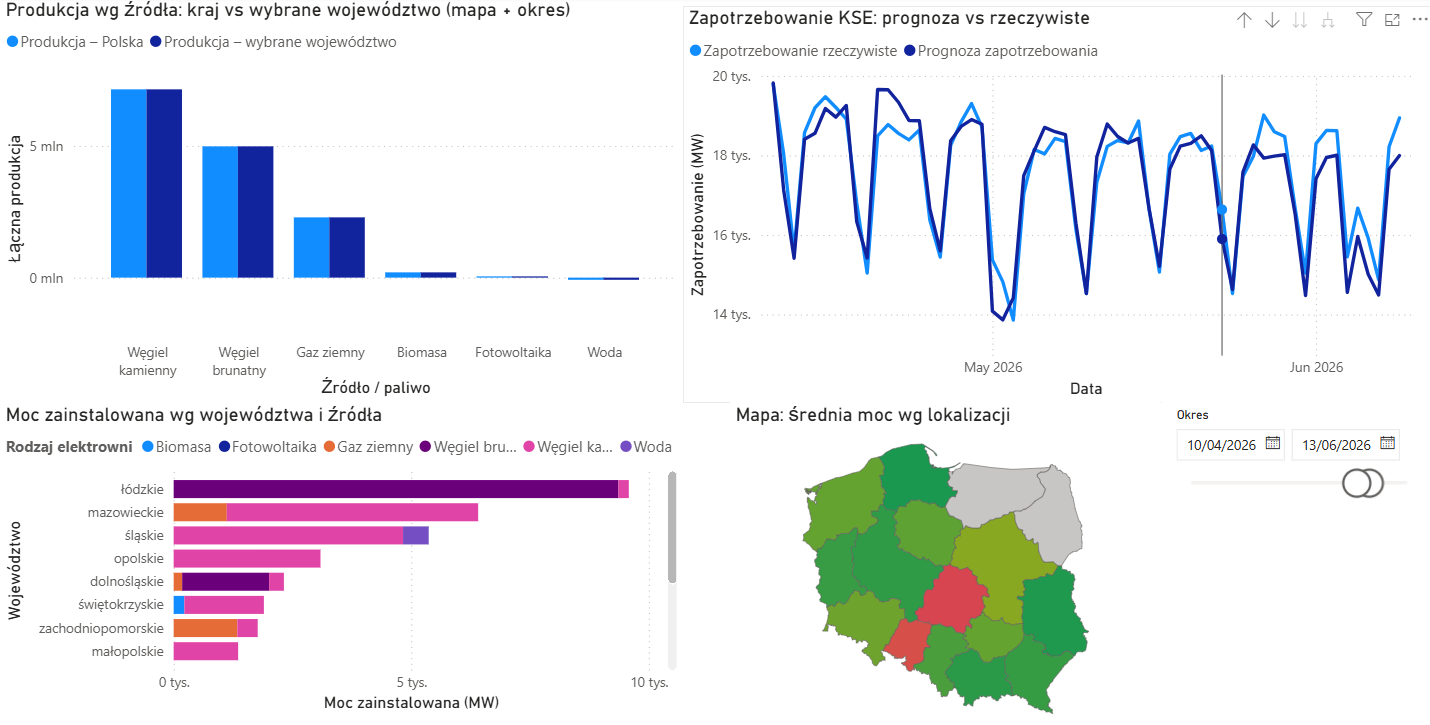
\includegraphics[width=\linewidth]{pbi_1_przeglad.png}
		\caption{Power BI - strona \textit{Przegląd} (fragmentator zakresu dat \textit{Okres} w prawym górnym rogu)}
	\end{figure}

	\subsection{Strona 2: Rynek i bilansowanie}
	Analiza rynkowa w trzech wykresach liniowych:
	\begin{itemize}
		\item \textit{Ceny i koszty bilansujące w czasie} - składowe cenowe CDSAC, CEB śr., CEN, COR i SK (w PLN),
		\item \textit{Zapotrzebowanie KSE vs produkcja największych elektrowni} - zapotrzebowanie rzeczywiste zestawione z miarą \texttt{Moc floty} (w MW),
		\item \textit{Rynkowa cena energii (RCE)} - przebieg średniej \texttt{rce\_cost} w PLN.
	\end{itemize}
	\begin{figure}[H]
		\centering
		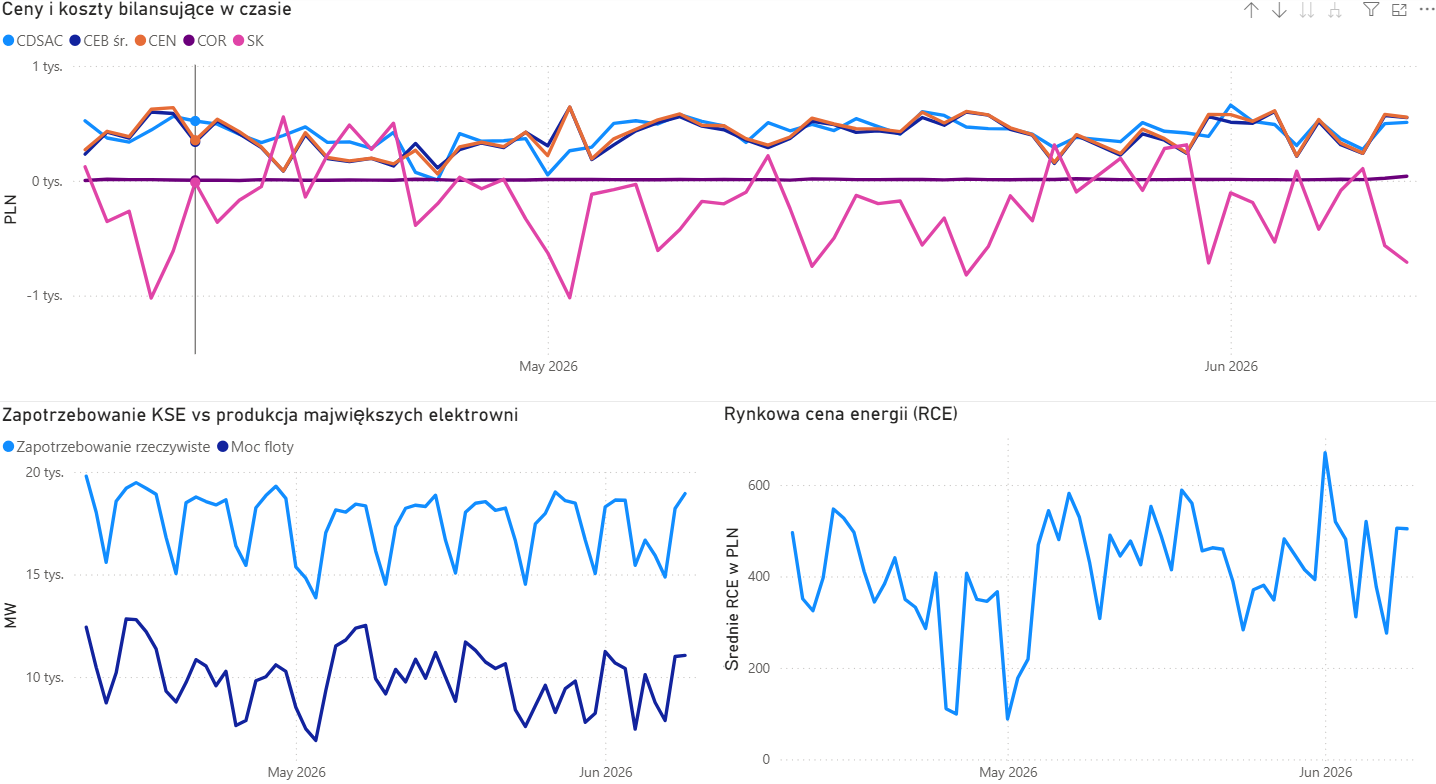
\includegraphics[width=\linewidth]{pbi_2_rynek.png}
		\caption{Power BI - strona \textit{Rynek i bilansowanie} (wykresy liniowe z hierarchią czasu umożliwiającą drążenie)}
	\end{figure}

	\subsection{Strona 3: Pogoda a produkcja}
	Sedno celu biznesowego - dwa wykresy punktowe wiążące produkcję z pogodą:
	\begin{itemize}
		\item \textit{Produkcja a temperatura (rozmiar = moc zainst., kolor = paliwo)} - średnia moc względem średniej temperatury, kolor wg kategorii paliwa, rozmiar punktu wg mocy zainstalowanej,
		\item \textit{Produkcja a ciśnienie (kolor = kod pogody)} - średnia moc względem średniego ciśnienia, kolor wg kodu zjawiska pogodowego.
	\end{itemize}
	\begin{figure}[H]
		\centering
		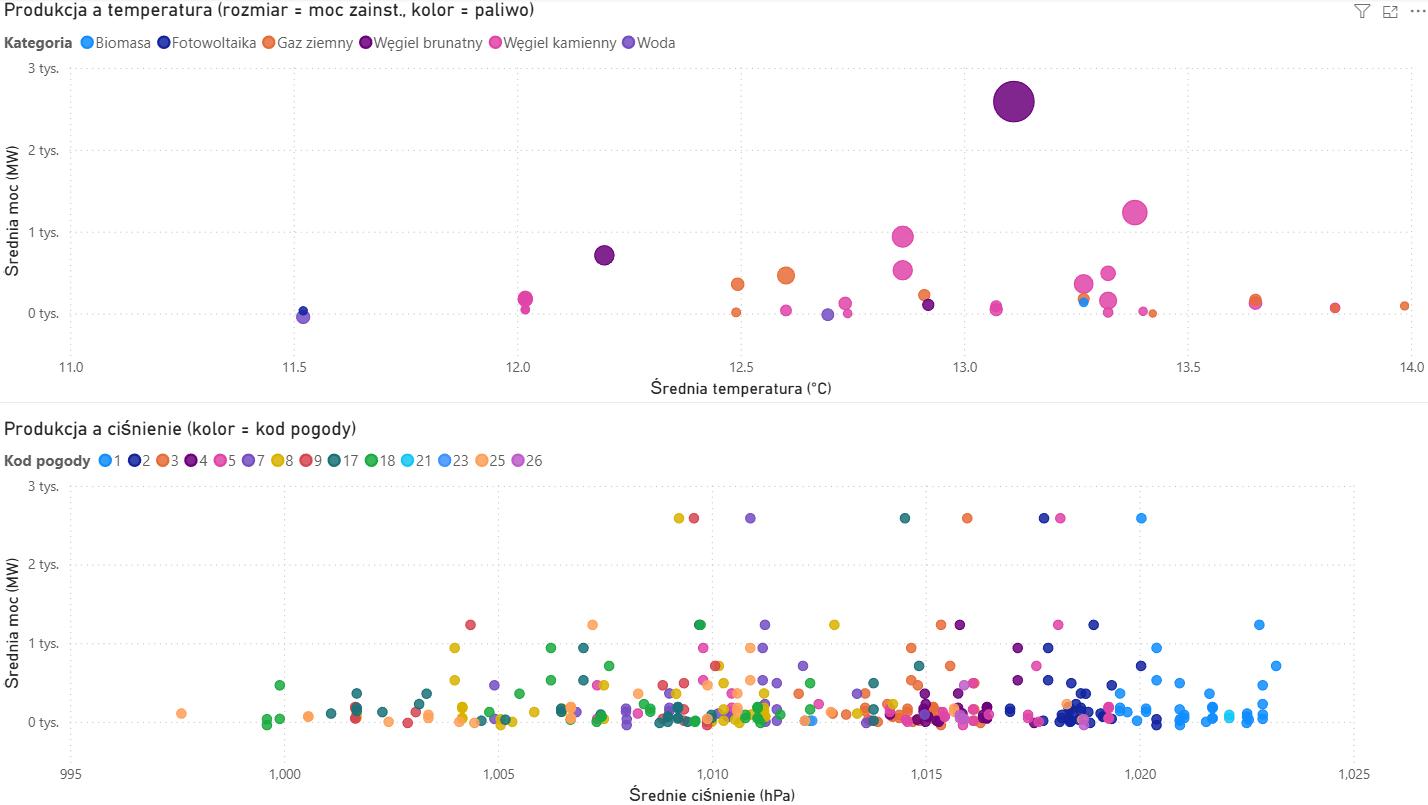
\includegraphics[width=\linewidth]{pbi_3_pogoda.png}
		\caption{Power BI - strona \textit{Pogoda a produkcja} (legendy kategorii paliwa i kodu pogody działają jako interaktywne filtry)}
	\end{figure}

	\subsection{Strona 4: Ceny i bilans}
	Powiązania cen z popytem i bilansem (podział \textit{Czy weekend}):
	\begin{itemize}
		\item \textit{Błąd prognozy (MW) wg Godzina} - wykres kolumnowy miary \texttt{Błąd prognozy (MW)} w przekroju godzin doby (największe odchylenia w godzinach okołopołudniowych),
		\item tabela przestawna średniej RCE w układzie godzina $\times$ dzień tygodnia (z sumami),
		\item \textit{Średni bilans mocy i średnie rce wg godziny} - wykres punktowy RCE względem bilansu mocy,
		\item \textit{Zależność średniej prawdziwego obciążenia (MW) i RCE (PLN) wg godziny} - wykres punktowy RCE względem rzeczywistego obciążenia.
	\end{itemize}
	\begin{figure}[H]
		\centering
		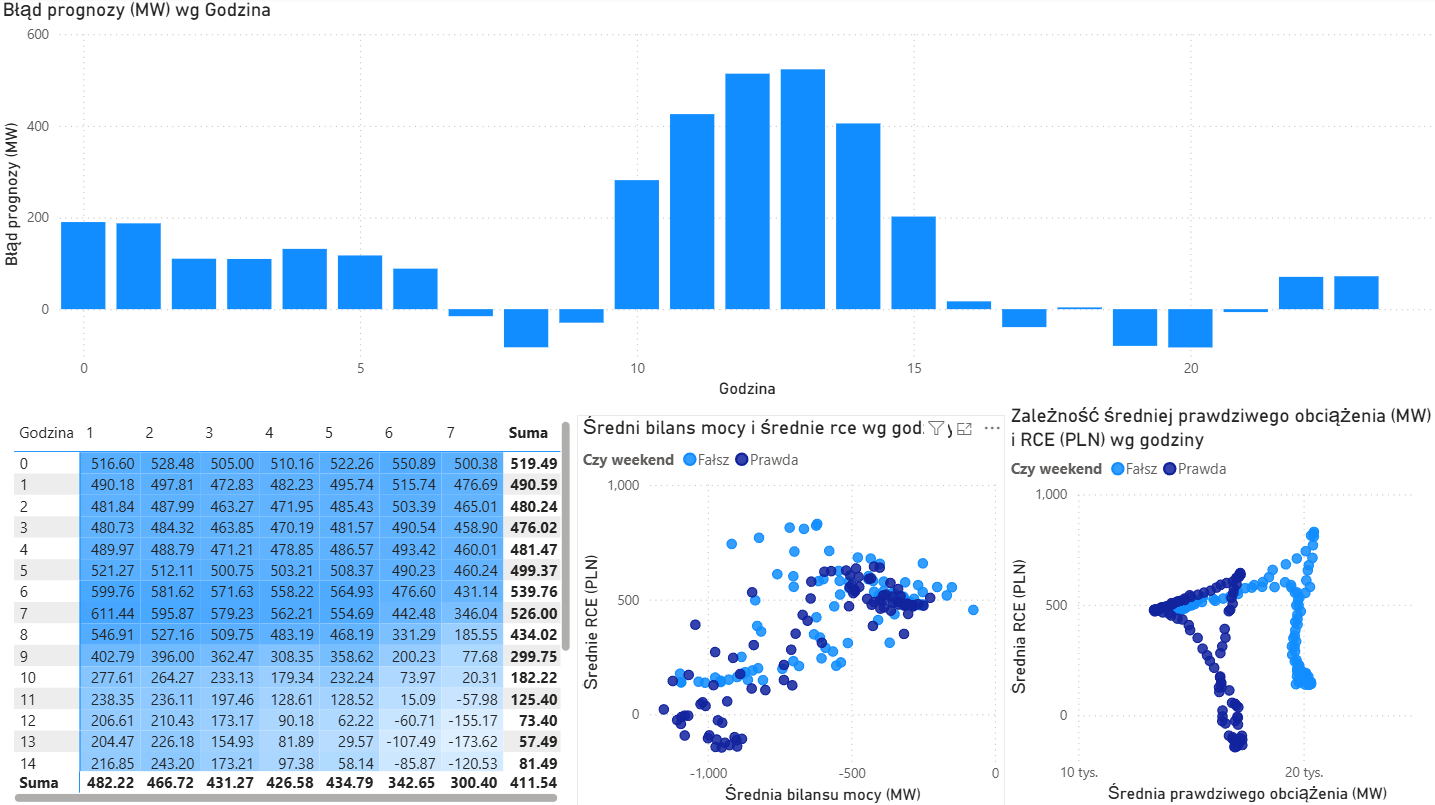
\includegraphics[width=\linewidth]{pbi_4_ceny.png}
		\caption{Power BI - strona \textit{Ceny i bilans} (podział serii wg legendy \textit{Czy weekend}: Fałsz/Prawda)}
	\end{figure}

	\subsection{Strona 5: Wzorce czasowe}
	Analiza sezonowości i profili dobowych:
	\begin{itemize}
		\item \textit{Współczynnik wykorzystania w czasie} - wykres kolumnowy miary \texttt{Współczynnik wykorzystania} z hierarchią drążenia miesiąc $\rightarrow$ tydzień $\rightarrow$ dzień tygodnia $\rightarrow$ godzina,
		\item \textit{Średnia prawdziwego obciążenia [MW] wg Dzień tygodnia} - wykres kolumnowy ujawniający wyższe obciążenie w dni robocze niż w weekend.
	\end{itemize}
	\begin{figure}[H]
		\centering
		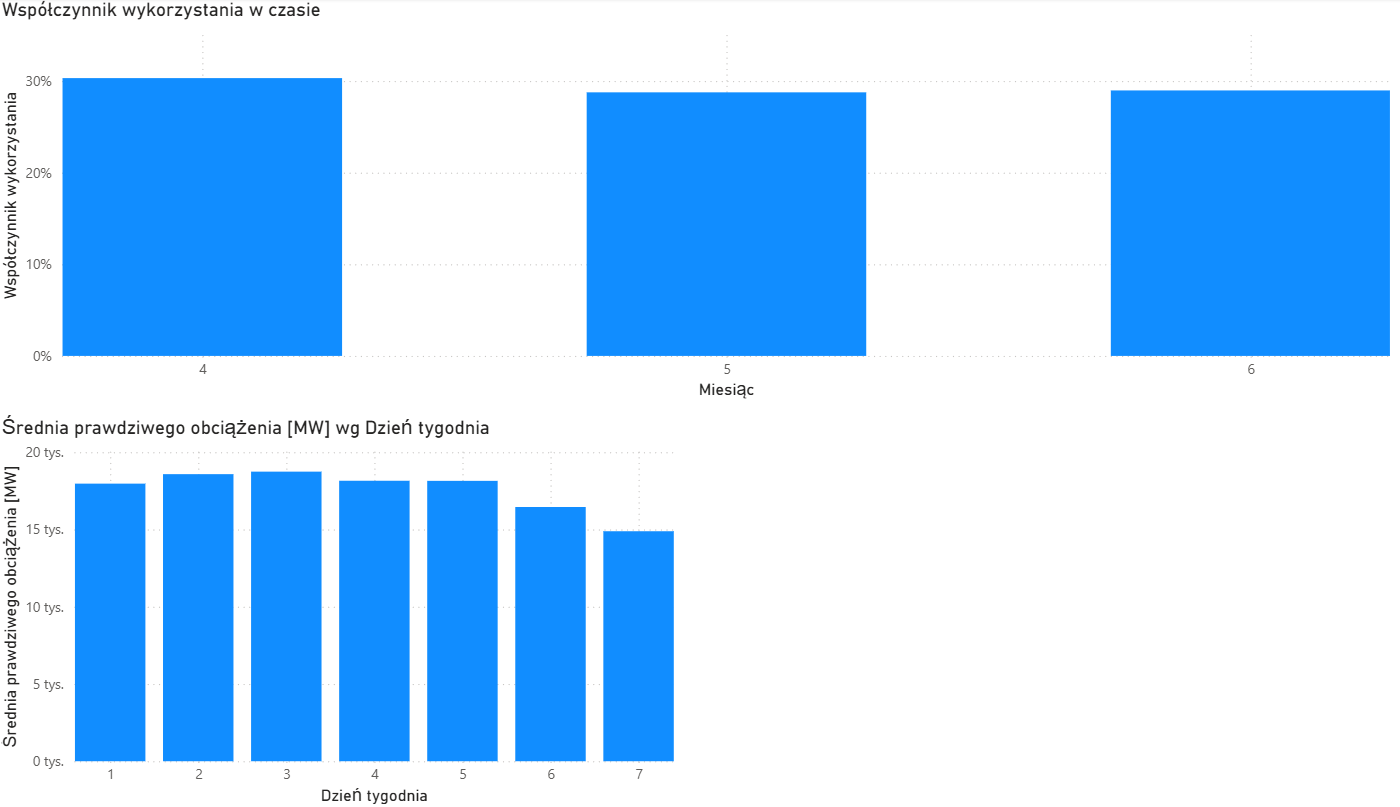
\includegraphics[width=\linewidth]{pbi_5_wzorce.png}
		\caption{Power BI - strona \textit{Wzorce czasowe}. Wykres \textit{Współczynnik wykorzystania w czasie} (u góry, wg miesiąca) ma hierarchię drążenia miesiąc $\rightarrow$ tydzień $\rightarrow$ dzień tygodnia $\rightarrow$ godzina}
	\end{figure}

	\subsection{Strona 6: Geografia i moce}
	Ujęcie przestrzenne i porównanie jednostek (fragmentator \textit{Kategoria}):
	\begin{itemize}
		\item \textit{Moc zainstalowana elektrowni wg lokalizacji i paliwa [MW]} - mapa punktowa na podkładzie geograficznym, rozmiar wg mocy zainstalowanej, kolor wg kategorii,
		\item \textit{Współczynnik wykorzystania wg paliwa} - wykres kolumnowy (najwyższy dla Biomasy, najniższy dla Wody),
		\item \textit{Moc zainstalowana wg województw i paliwa [MW]} - skumulowany wykres kolumnowy,
		\item \textit{Średnia produkcja wg elektrowni [MW]} - wykres słupkowy rankingowy (m.in. Bełchatów, Opole, Kozienice 2, Turów, Kozienice 1, Jaworzno 2 JWCD, Gryfino, Połaniec).
	\end{itemize}
	\begin{figure}[H]
		\centering
		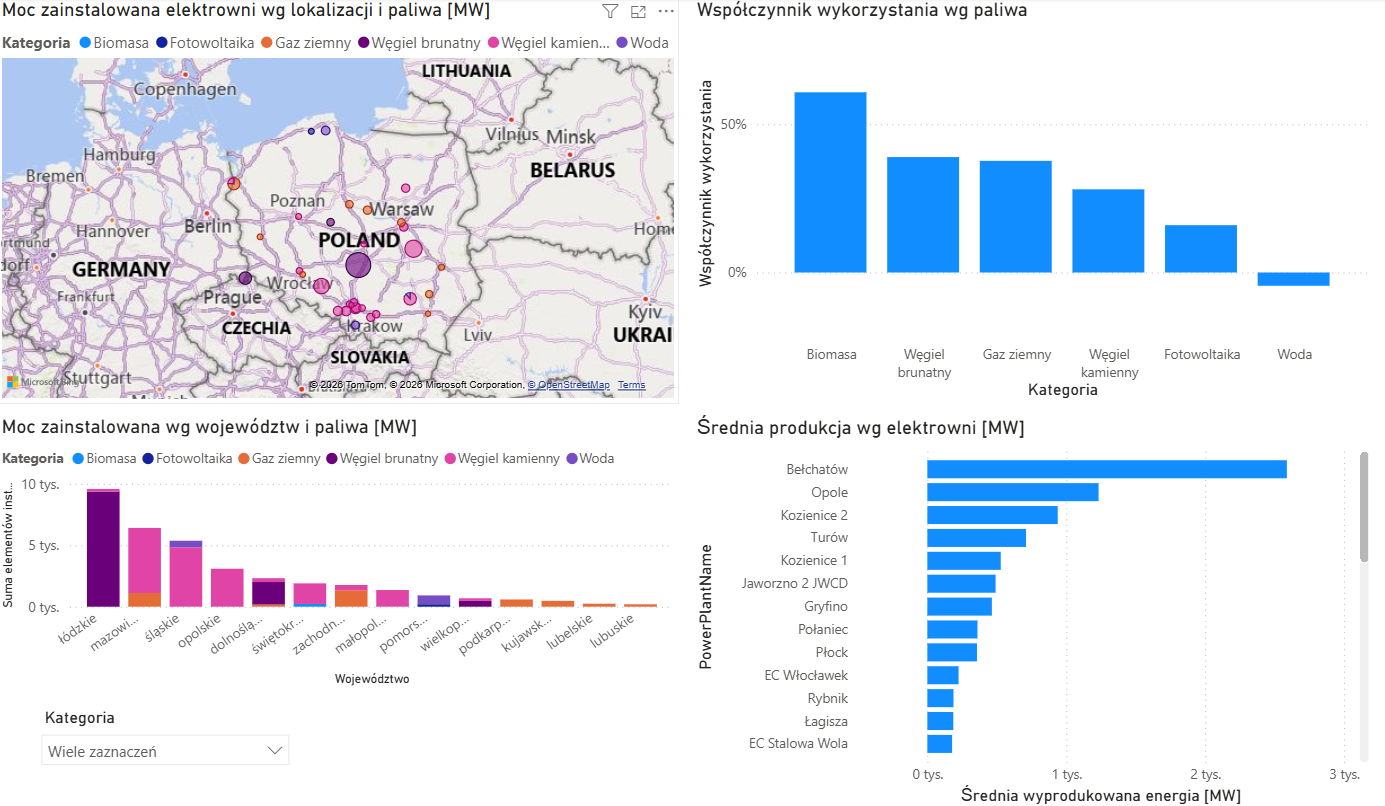
\includegraphics[width=\linewidth]{pbi_6_geografia.png}
		\caption{Power BI - strona \textit{Geografia i moce} (fragmentator \textit{Kategoria} z wielokrotnym wyborem w lewym dolnym rogu)}
	\end{figure}

	\subsection{Strona 7: Pogoda a moc (kosze)}
	Strona analityczna poświęcona bezpośrednio zależności średniej produkcji elektrowni od warunków pogodowych. Zawiera trzy wykresy kolumnowe grupowane (świadomie zamiast wykresów punktowych), w których oś X stanowią przedziały (kosze) wartości pogodowej, legendę - kategoria paliwa, a wysokość słupka - średnią moc:
	\begin{itemize}
		\item \textit{Średnia moc wg temperatury (kosze 2 °C)} - przedziały temperatury co 2 °C,
		\item \textit{Średnia moc wg punktu rosy (kosze 2 °C)} - przedziały punktu rosy co 2 °C,
		\item \textit{Średnia moc wg prędkości wiatru (kosze 1 m/s)} - przedziały prędkości wiatru co 1 m/s (oś przycięta do 40 m/s).
	\end{itemize}
	Przedziały utworzono mechanizmem grupowania (binning) Power BI. Kluczowym elementem jest autorska miara DAX \texttt{Średnia moc wg pogody}, która za pomocą funkcji \texttt{TREATAS} przenosi kontekst pomiaru pogodowego (\texttt{TimeId} i \texttt{PowerPlantId} z \texttt{FactWeather}) na wymiary \texttt{DimTime} i \texttt{DimPowerPlant}. Dzięki temu średnia z \texttt{FactPowerPlantOutput[Power]} reaguje na kosz pogodowy mimo jednokierunkowych relacji między tabelami faktów (bez tego słupki byłyby płaskie - pokazywałyby średnią globalną). Przygotowano także miary odchylenia standardowego i jego granic (\texttt{Odch std moc pogoda}, \texttt{Moc górna/dolna pogoda}), Power BI nie udostępnia jednak słupków błędu dla wykresu kolumnowego z legendą, więc nie zostały one naniesione. Widoczny jest spadek średniej mocy przy wysokich temperaturach oraz ujemne wartości dla kategorii Woda (praca pompowa elektrowni szczytowo-pompowych). Kosze temperatury i punktu rosy ustawiono na 2 °C (zamiast pierwotnych 0,5 °C) dla lepszej czytelności, a oś prędkości wiatru przycięto do 40 m/s, pomijając wizualnie pojedyncze wartości odstające źródła. Osie opisano jednostkami: oś X - °C (temperatura, punkt rosy) lub m/s (prędkość wiatru), oś Y - MW (średnia moc).
	\begin{figure}[H]
		\centering
		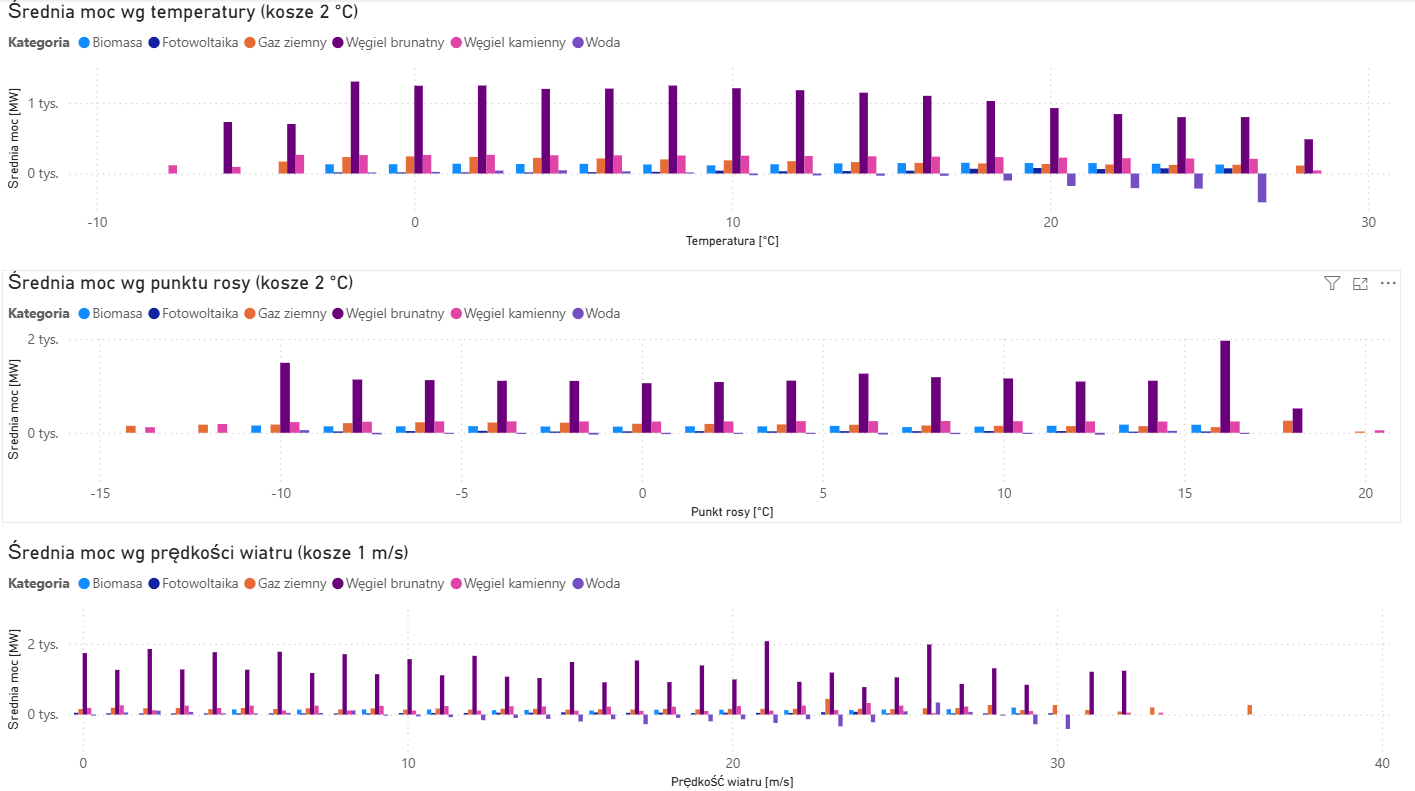
\includegraphics[width=\linewidth]{pbi_7_pogoda.png}
		\caption{Power BI - strona \textit{Pogoda a moc (kosze)}: średnia moc w przedziałach temperatury, punktu rosy i prędkości wiatru, w podziale na kategorię paliwa}
	\end{figure}

	\subsection{Interaktywność: fragmentatory i drążenie (drill-down)}
	Raport jest interaktywny - poniżej zestawiono dostępne opcje wyboru i drążenia oraz miejsca ich występowania:
	\begin{itemize}
		\item \textbf{Fragmentator \textit{Okres}} (zakres dat) - strona \textit{Przegląd}, prawy górny róg, ogranicza zakres czasowy wszystkich wizualizacji strony (domyślnie 10.04.2026-13.06.2026).
		\item \textbf{Fragmentator \textit{Kategoria}} (rodzaj elektrowni, tryb \textit{Wiele zaznaczeń}) - strona \textit{Geografia i moce}, lewy dolny róg, pozwala zawęzić analizę do wybranych paliw.
		\item \textbf{Drążenie hierarchii czasu} (drill-down) - wykres \textit{Współczynnik wykorzystania w czasie} (strona \textit{Wzorce czasowe}) oraz wykresy liniowe na stronach \textit{Przegląd} i \textit{Rynek i bilansowanie}: hierarchia miesiąc $\rightarrow$ tydzień $\rightarrow$ dzień tygodnia $\rightarrow$ godzina. Drążenie uruchamia się przyciskami w prawym górnym rogu wizualizacji (strzałka w dół - tryb drążenia, podwójna strzałka - przejście na niższy poziom dla wszystkich kategorii).
		\item \textbf{Podział wg legendy \textit{Czy weekend}} (Fałsz/Prawda) - wykresy punktowe na stronie \textit{Ceny i bilans}, rozróżnia dni robocze i weekend.
		\item \textbf{Interaktywne legendy} - kliknięcie pozycji legendy (kategoria paliwa, kod pogody) wyróżnia wybraną serię na stronach \textit{Przegląd}, \textit{Pogoda a produkcja} i \textit{Geografia i moce}.
		\item \textbf{Filtrowanie krzyżowe (cross-filtering)} - kliknięcie elementu jednej wizualizacji (np. województwa, paliwa lub elektrowni) automatycznie filtruje pozostałe wizualizacje strony, na tej zasadzie działa zestawienie \textit{kraj vs wybrane województwo} na stronie \textit{Przegląd}.
	\end{itemize}

	\medskip
	\noindent Kontrola jakości i kompletności ładowań realizowana jest w warstwie SQL (tabela \texttt{dq.CheckResults} oraz schemat \texttt{audit}, sekcja \ref{sec:dq}), niezależnie od raportów analitycznych Power BI.

	\section{Załączniki}

	Do raportu dołączone są artefakty implementacji znajdujące się w repozytorium projektu:
	\begin{itemize}
		\item \textbf{Skrypt modelu hurtowni}: \texttt{sql\_help/00\_Create\_PowerDWH\_empty.sql} - baza, schematy \texttt{etl}/\texttt{stg}, tabele wymiarów, faktów i staging, klucze obce, indeksy oraz procedura \texttt{etl.usp\_Load\_DimPowerPlant} (jej aktualna wersja również w \texttt{SCD\_2\_DimPowerPlant.sql}).
		\item \textbf{Skrypty kontroli jakości i audytu}: \texttt{sql\_help/DataQuality\_checks.sql}, \texttt{sql\_help/PostLoad\_checks.sql} oraz \texttt{sql\_help/Audit\_setup.sql} (schemat \texttt{audit}: \texttt{EtlRun}/\texttt{EtlStep}, widok \texttt{vLastRun}).
		\item \textbf{Raport Power BI}: \texttt{business.pbix} (siedem stron analitycznych) wraz z plikami granic województw \texttt{poland\_voivodeships\_pl.geojson}.
		\item \textbf{Skrypty ETL (Python)}: \texttt{extract\_powerplant.py}, \texttt{extract\_poland\_energy.py}, \texttt{extract\_power\_output.py}, \texttt{extract\_weather.py}, \texttt{DimTimeloader.py}, \texttt{load\_range.py} (orkiestrator) oraz \texttt{requirements.txt}.
		\item \textbf{Pakiety SSIS}: \texttt{Master.dtsx}, \texttt{Load\_DimTime.dtsx}, \texttt{Load\_DimPowerPlant.dtsx}, \texttt{Load\_FactPolandEnergy.dtsx}, \texttt{Load\_FactPowerPlantOutput.dtsx}, \texttt{Load\_FactWeather.dtsx}.
		\item \textbf{Dane referencyjne}: \texttt{powerplant\_meta.csv}, \texttt{DimTime.csv}, pliki GeoJSON województw.
	\end{itemize}
\end{document}
